
%(BEGIN_QUESTION)
% Copyright 2007, Tony R. Kuphaldt, released under the Creative Commons Attribution License (v 1.0)
% This means you may do almost anything with this work of mine, so long as you give me proper credit

Many industries produce flammable waste products that may be used as fuel in furnaces, steam boilers, and process heaters.  Obviously, if one may use a waste fuel instead of paying for natural gas or fuel oil, a double economic benefit awaits: not only do you pay less for energy, but you rid yourself of a waste product ordinarily costing money to dispose of.

Waste fuel flow, however, is often unsteady.  Combustion processes usually cannot run solely on waste fuel because the supply is liable to change.  For this reason, heat processes using waste fuels supplement their waste fuel sources with purchased fuels such as gas, oil, and/or coal.  This requires a control system to manage the mix of waste and purchased fuel.  Here is an example:

$$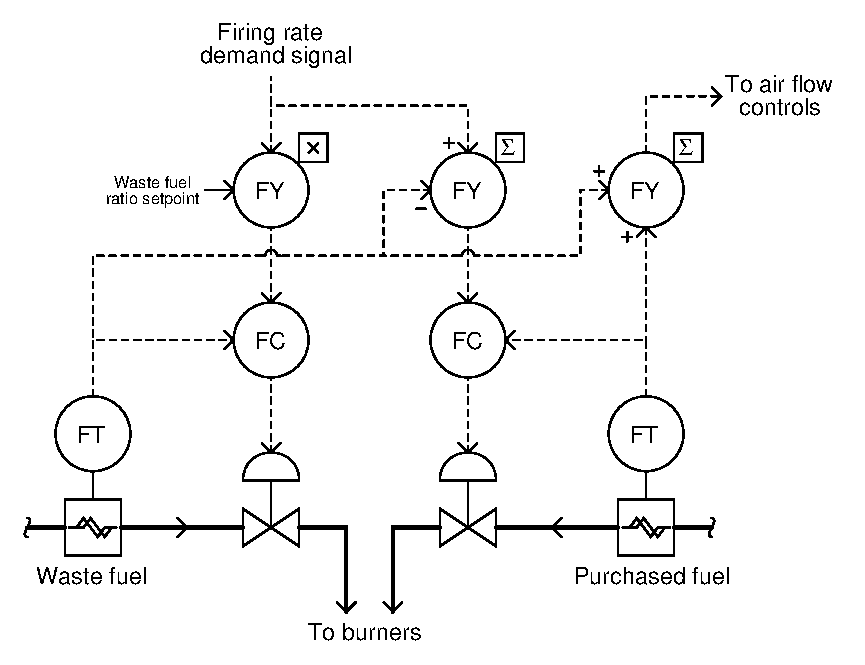
\includegraphics[width=15.5cm]{i01832x01.eps}$$

After examining this control scheme, answer the following questions:

\begin{itemize}
\item{} Which controller inputs are process variables (PVs), and which are setpoints (SPs)?
\item{} What is the purpose of the multiplier function?
\item{} Why would the waste fuel ratio setpoint ever be set at a value other than unity (100\%)?
\item{} What is the purpose of the subtractor function?
\item{} What is the purpose of the summer function?
\item{} How would the control system respond if the waste fuel source suddenly ran out, so that waste fuel flow dropped to zero?
\end{itemize}

\vskip 20pt \vbox{\hrule \hbox{\strut \vrule{} {\bf Suggestions for Socratic discussion} \vrule} \hrule}

\begin{itemize}
\item{} Assuming signal-to-open control valves, determine the necessary actions of each controller in this system, and mark their PV and SP inputs accordingly with ``+'' and ``$-$'' symbols.
\item{} How would the control system respond if the purchased fuel source suddenly ran out, so that purchased fuel flow dropped to zero?
\item{} For those who have studied flowmeters, what type of flow-measuring instruments are used in this control system, and what benefit(s) do they hold over the more standard orifice plate and DP cell variety?
\item{} Explain what will happen in this system if the waste fuel flow transmitter fails with a low signal.
\item{} Explain what will happen in this system if the waste fuel flow transmitter fails with a high signal.
\item{} Explain what will happen in this system if the purchased fuel flow transmitter fails with a low signal.
\item{} Explain what will happen in this system if the purchased fuel flow transmitter fails with a high signal.
\end{itemize}

\underbar{file i01832}
%(END_QUESTION)





%(BEGIN_ANSWER)

\noindent
{\bf Partial answer:}

\begin{itemize}
\item{} What is the purpose of the multiplier function? {\it To establish a target value for percentage of fuel that is waste fuel.}
\vskip 10pt
\item{} Why would the waste fuel ratio setpoint ever be set at a value other than unity (100\%)? {\it Perhaps the waste fuel does not burn clean, and 100\% usage would create emissions problems, so it must be ``diluted'' at a prescribed ratio with clean, purchased fuel.}
\vskip 10pt
\item{} How would the control system respond if the waste fuel source suddenly ran out, so that waste fuel flow dropped to zero? {\it The purchased fuel valve would open as necessary to maintain the same total fuel flow as directed by the firing rate demand signal.}
\end{itemize}


%(END_ANSWER)





%(BEGIN_NOTES)

\begin{itemize}
\item{} Which controller inputs are process variables (PVs), and which are setpoints (SPs)? {\it The signals coming from transmitters are PVs, while the other signals entering controllers are SPs.}
\vskip 10pt
\item{} What is the purpose of the multiplier function? {\it To establish a target value for percentage of fuel that is waste fuel.}
\vskip 10pt
\item{} Why would the waste fuel ratio setpoint ever be set at a value other than unity (100\%)? {\it Perhaps the waste fuel does not burn clean, and 100\% usage would create emissions problems, so it must be ``diluted'' at a prescribed ratio with clean, purchased fuel.}
\vskip 10pt
\item{} What is the purpose of the subtractor function? {\it This function generates a setpoint for the purchased fuel flow controller.}
\vskip 10pt
\item{} What is the purpose of the summer function? {\it This function calculates total fuel flow, waste + purchased.}
\vskip 10pt
\item{} How would the control system respond if the waste fuel source suddenly ran out, so that waste fuel flow dropped to zero? {\it The purchased fuel valve would open as necessary to maintain the same total fuel flow as directed by the firing rate demand signal.}
\end{itemize}

\vskip 10pt

The flowmeters used in this control system are {\it Coriolis} mass flow transmitters.  These instruments provide inherently true mass flow measurement, not volumetric measurement.  This is especially useful when the waste fuel in question varies in mass density, and thus in energy content per unit volume (energy density).

%INDEX% Control, strategies: waste fuel flow control system
%INDEX% Process: waste fuel flow control

%(END_NOTES)


